\documentclass{physlab}

\begin{document}
\begin{titlepage}
\center % Center everything on the page
 
%----------------------------------------------------------------------------------------
%	HEADING SECTIONS
%----------------------------------------------------------------------------------------

\textsc{\LARGE Московский\\[-0.2cm]Физико-Технический Институт\\[0.1cm]\large (государственный университет)}\\[1.5cm] % Name of your university/college
\textsc{\Large Кафедра общей физики}\\[0.1cm] % Major heading such as course name
\textsc{\large Лабораторная работа № 3.1.1}\\[0.5cm] % Minor heading such as course title

%----------------------------------------------------------------------------------------
%	TITLE SECTION
%----------------------------------------------------------------------------------------

\HRule
\\[0.6cm]
{ \huge \bfseries Магнитометр}
\\[0.3cm] % Title of your document
\HRule
\\[1.5cm]


 
%----------------------------------------------------------------------------------------
%	AUTHOR SECTION
%----------------------------------------------------------------------------------------

\begin{minipage}[t]{0.48\textwidth}
	\begin{flushleft} \large
		\textsf{Студент}\bigskip
		
		\tline{(имя)}{30mm} \tline{(фамилия)}{45mm} \\[5mm]
		\underline{\hspace{30mm}} группа
	\end{flushleft}
\end{minipage}
\hfill
\begin{minipage}[t]{0.48\textwidth}
	\begin{flushright} \large
		\textsf{Преподаватель}\bigskip
		
		\tline{(имя)}{30mm} \tline{(отчество)}{45mm} \\[5mm]
		\tline{(фамилия)}{45mm}
	\end{flushright}
\end{minipage}

\begin{bottompar}
	\begin{center}
		
\includegraphics[width = 80 mm]{logo.jpg}
	\end{center}
	\tline{(дата)}{80mm}

\end{bottompar}
\vfill % Fill the rest of the page with whitespace

\end{titlepage}

\paragraph{Цель работы:} изучить влияние активного сопротивления, индуктивности и ёмкости на~сдвиг фаз между током и~напряжением в~цепи переменного тока.

\section{Экспериментальная установка}

\begin{figure}[H]\centering
    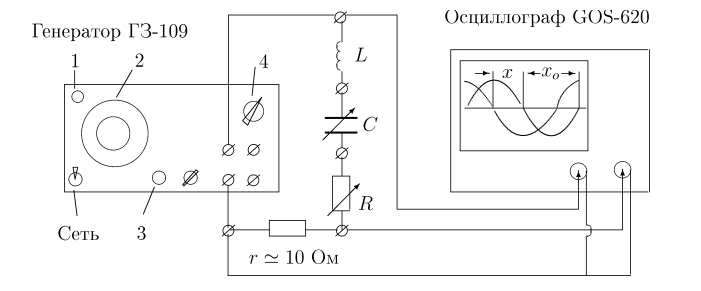
\includegraphics[width=0.85\tw]{t}
\end{figure}
\vspace{-2ex}
\begin{align*}
    R_L &= \val & \text{при}~\nu &= \val \\[1ex]
    L &= \val \\[1ex]
    r &= \val \\[1ex]
    C &= \val \\[1ex]
    \nu &= \val
\end{align*}

\subsection*{RC-цепь}
Ток, текущий через RC"=цепочку, пропорционален напряжению на резисторе, и опережает напряжение на конденсаторе по фазе на $\pi/2$. В таком простом случае метод векторных диаграмм даёт простой результат для зависимости сдвига фаз от $R$:
$$\tg \varphi = \frac{1}{\Omega R C}.$$
\begin {figure}[H]
\begin{center}
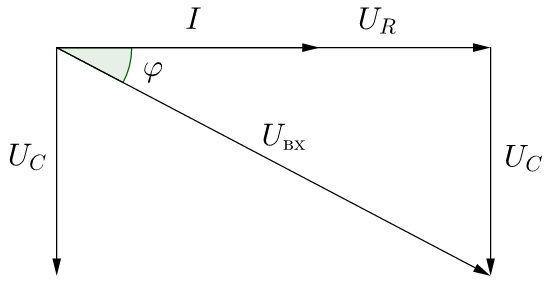
\includegraphics[width=0.6\tw]{rcd}
\end{center}
\end {figure}

\subsection*{RL-цепь}
Рассмотрение этого случая аналогично предыдущему. Импеданс катушки равен $Z_2 = j\omega L$, поэтому ток отстаёт по фазе от напряжения, и расчётная формула приобретает вид
$$\tg \varphi = \frac{\omega L}{R_{\sum}}.$$
К сопротивлению калибровочного резистора и резистора $R$ добавится активное сопротивление катушки:
$$R_{\sum} = R+r+R_L,$$
где $R_L$ -- активное сопротивление катушки.

\subsection*{RCL-цепь}

\vspace{-1.75ex}
Комплексный импеданс RCL-цепочки $Z=R+j\omega L - \dfrac{j}{\omega C}$.
\vspace{.75\parskip}

Сдвиг фаз между током и напряжением получим, взяв аргумент $Z$:
$$\tg\varphi = \frac{\omega L - 1/(\omega C)}{R} = Q\frac{\left(\omega/\omega_0\right)^2 - 1}{\omega/\omega_0} = Q\frac{(1+x)^2-1}{1+x} \simeq 2x Q,$$
где $x \equiv \Delta \omega / \omega_0 = \Delta \nu / \nu_0$.
В последнем переходе пренебрегаем степенями~$x$ выше первой.
Измерив ширину графика $w=2x$ на высоте $\varphi = \pi / 4\ (\tg\varphi = 1)$, можем непосредственно определить добротность контура:
$$Q = \frac{1}{w}.$$

\subsection*{Фазовращатель}

\vspace{-7.5mm}
\begin{minipage}{.65\tw}
    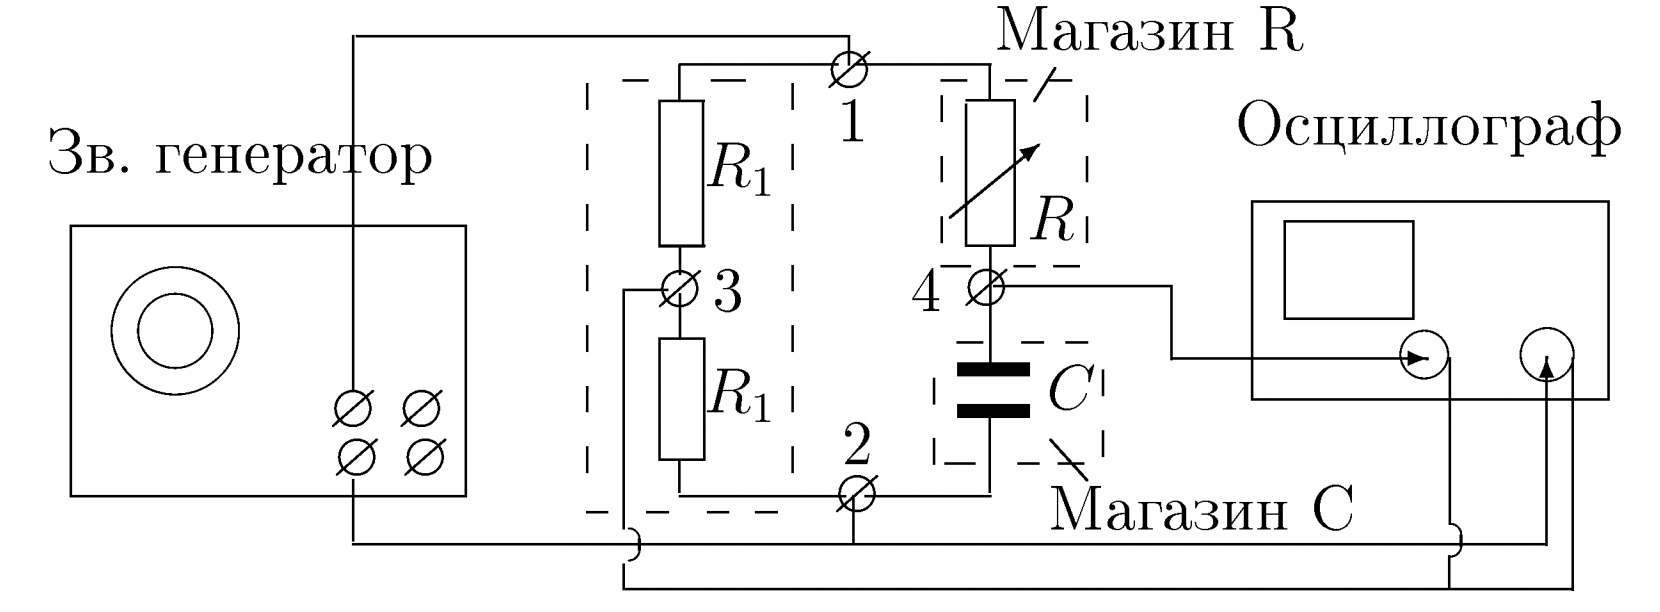
\includegraphics[width=\lw]{phase}
\end{minipage}
\hfill
\begin{minipage}{.32\tw}
    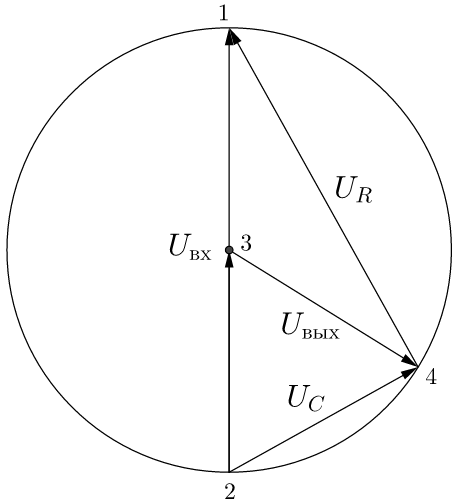
\includegraphics[width=\lw]{diagramphase}
\end{minipage}\smallskip

Разность фаз равна $\pi /2$, когда медиана $\overline{34}$ в то же время является и высотой, т.\,е. когда $\triangle 124$ -- равнобедренный, откуда \emph{что?}

\section{Работа и измерения}

\subsection*{RC-цепь}

$$X_1 = \dfrac{1}{2 \pi \nu C} = \val$$

\begin{table}[H]
\centering
\begin{tabular}{|c|c|c|c|c|c|c|}
\hline
$R$ & $x$ & $x_0$ & $\varphi$ & $\tg \varphi$ & $R_{\Sigma}$ & $1/(R_{\Sigma} \Omega C)$ \\ \hline
\val    &    \val   &   \val    &   \val    &   \val    &   \val    &   \val    \\ \hline
\val    &    \val   &   \val    &   \val    &   \val    &   \val    &   \val    \\ \hline
\val    &    \val   &   \val    &   \val    &   \val    &   \val    &   \val    \\ \hline
\val    &    \val   &   \val    &   \val    &   \val    &   \val    &   \val    \\ \hline
\val    &    \val   &   \val    &   \val    &   \val    &   \val    &   \val    \\ \hline
\val    &    \val   &   \val    &   \val    &   \val    &   \val    &   \val    \\ \hline
\val    &    \val   &   \val    &   \val    &   \val    &   \val    &   \val    \\ \hline
\val    &    \val   &   \val    &   \val    &   \val    &   \val    &   \val    \\ \hline
\val    &    \val   &   \val    &   \val    &   \val    &   \val    &   \val    \\ \hline
\val    &    \val   &   \val    &   \val    &   \val    &   \val    &   \val    \\ \hline
\val    &    \val   &   \val    &   \val    &   \val    &   \val    &   \val    \\ \hline
\val    &    \val   &   \val    &   \val    &   \val    &   \val    &   \val    \\ \hline
\end{tabular}
\caption{Полученные значения в RC-цепи}
\end{table}

\begin{figure}[b!]\centering
	
\includegraphics[width=.65\tw]{foo}
	\caption{График зависимости $\tg \varphi = f[1/ \Omega C R_{\Sigma}]$}
\end{figure}
\clearpage

\subsection*{RL-цепь}
\[X_2 = 2 \pi \nu L = \val \]

\begin{table}[H]
\centering
\begin{tabular}{|c|c|c|c|c|c|c|}
\hline
$R $ & $x$  & $x_0$ & $\varphi$ & $\tg \varphi$ & $R_{\Sigma}$ & $\Omega L/ R_{\Sigma} $ \\ \hline
\val & \val & \val  & \val      & \val          & \val         & \val                  \\ \hline
\val & \val & \val  & \val      & \val          & \val         & \val                  \\ \hline
\val & \val & \val  & \val      & \val          & \val         & \val                  \\ \hline
\val & \val & \val  & \val      & \val          & \val         & \val                  \\ \hline
\val & \val & \val  & \val      & \val          & \val         & \val                  \\ \hline
\val & \val & \val  & \val      & \val          & \val         & \val                  \\ \hline
\val & \val & \val  & \val      & \val          & \val         & \val                  \\ \hline
\val & \val & \val  & \val      & \val          & \val         & \val                  \\ \hline
\val & \val & \val  & \val      & \val          & \val         & \val                  \\ \hline
\val & \val & \val  & \val      & \val          & \val         & \val                  \\ \hline
\val & \val & \val  & \val      & \val          & \val         & \val                  \\ \hline
\val & \val & \val  & \val      & \val          & \val         & \val                  \\ \hline
\end{tabular}
\caption{Полученные значения в RL-цепи}
\end{table}

\begin{figure}[b!]\centering
	
\includegraphics[width=.65\tw]{foo}
	\caption{График зависимости $\tg \varphi = f[\Omega L / R_{\Sigma}]$}
\end{figure}

\subsection*{RCL-цепь}

\begin{table}[H]
\centering
\begin{tabular}{|c|c|c|c|c|c|}
\hline
Сопротивление & $\nu, \text{кГц}$ & $x_0$ & $x$ & $\varphi$ & $\nu/\nu_0$ \\ \hline
\multirow{10}{*}{$R = 0 \text{ Ом}$}     & \val            & \val   & \val & \val   & \val      \\ \cline{2-6} 
                                         & \val            & \val   & \val & \val   & \val      \\ \cline{2-6}
                                         & \val            & \val   & \val & \val   & \val      \\ \cline{2-6}
                                         & \val            & \val   & \val & \val   & \val      \\ \cline{2-6}
                                         & \val            & \val   & \val & \val   & \val      \\ \cline{2-6}
                                         & \val            & \val   & \val & \val   & \val      \\ \cline{2-6}
                                         & \val            & \val   & \val & \val   & \val      \\ \cline{2-6}
                                         & \val            & \val   & \val & \val   & \val      \\ \cline{2-6}
                                         & \val            & \val   & \val & \val   & \val      \\ \cline{2-6}
                                         & \val            & \val   & \val & \val   & \val      \\ \hline
\multirow{12}{*}{$R = 100 \text{ Ом}$}   & \val            & \val   & \val & \val   & \val      \\ \cline{2-6} 
                                         & \val            & \val   & \val & \val   & \val      \\ \cline{2-6}
                                         & \val            & \val   & \val & \val   & \val      \\ \cline{2-6}
                                         & \val            & \val   & \val & \val   & \val      \\ \cline{2-6}
                                         & \val            & \val   & \val & \val   & \val      \\ \cline{2-6}
                                         & \val            & \val   & \val & \val   & \val      \\ \cline{2-6}
                                         & \val            & \val   & \val & \val   & \val      \\ \cline{2-6}
                                         & \val            & \val   & \val & \val   & \val      \\ \cline{2-6}
                                         & \val            & \val   & \val & \val   & \val      \\ \cline{2-6}
                                         & \val            & \val   & \val & \val   & \val      \\ \hline
\end{tabular}
\caption{Полученные значения при изучении зависимости фазы от $\dfrac{\nu}{\nu_0}$}
\end{table}

\vspace{-1cm}
\begin{align*}
    C &= \val \\[1ex]
    L &= \val \\[1ex]
    \nu_0 &= \val    
\end{align*}

% dirty hack, i'm too lazy
Из графика $R = 0$ Ом\hfill добротность $Q_{0}= $\hspace{8.29cm}~

\vspace{-\parskip}
Из графика $R = 100$ Ом \hfill добротность $Q_{100}= $\hspace{8cm}~

Можно рассчитать добротность, выразив её через параметры цепочки:
$Q = \dfrac{1}{R} \sqrt{\dfrac{L}{C}}$.
\begin{align*}
    Q_{\text{теор, 0}} &= \val \\[1ex]
    Q_{\text{теор, 100}} &= \val 
\end{align*}

\begin {figure}[p]
	\begin{center}
		
\includegraphics[width=0.75\tw]{foo}
		\caption{График зависимости $\varphi = f[\nu/\nu_0] \text{ при $R = 0$ Ом}$}
	\end{center}
\end {figure}

\begin {figure}[p]
	\begin{center}
		
\includegraphics[width=0.75\tw]{foo}
		\caption{График зависимости $\varphi = f[\nu/\nu_0] \text{ при $R = 100$ Ом}$}
	\end{center}
\end {figure}
\clearpage


\section{Вывод}

В настоящей лабораторной работе была изучена зависимость сдвига фаз между током и~напряжением от сопротивления в цепи в RC- и RL-цепях. Была определена добротность колебательного контура, снята зависимость сдвига фаз от частоты вблизи резонанса.

~\\[-1ex]\hrule~\\[1ex]\hrule~\\[1ex]\hrule~\\[1ex]\hrule~\\[1ex]\hrule~\\[1ex]\hrule~\\[1ex]\hrule~\\[1ex]\hrule

\end{document}